\documentclass{article}
\usepackage{tikz}
\usepackage{amsmath,amssymb}

\begin{document}

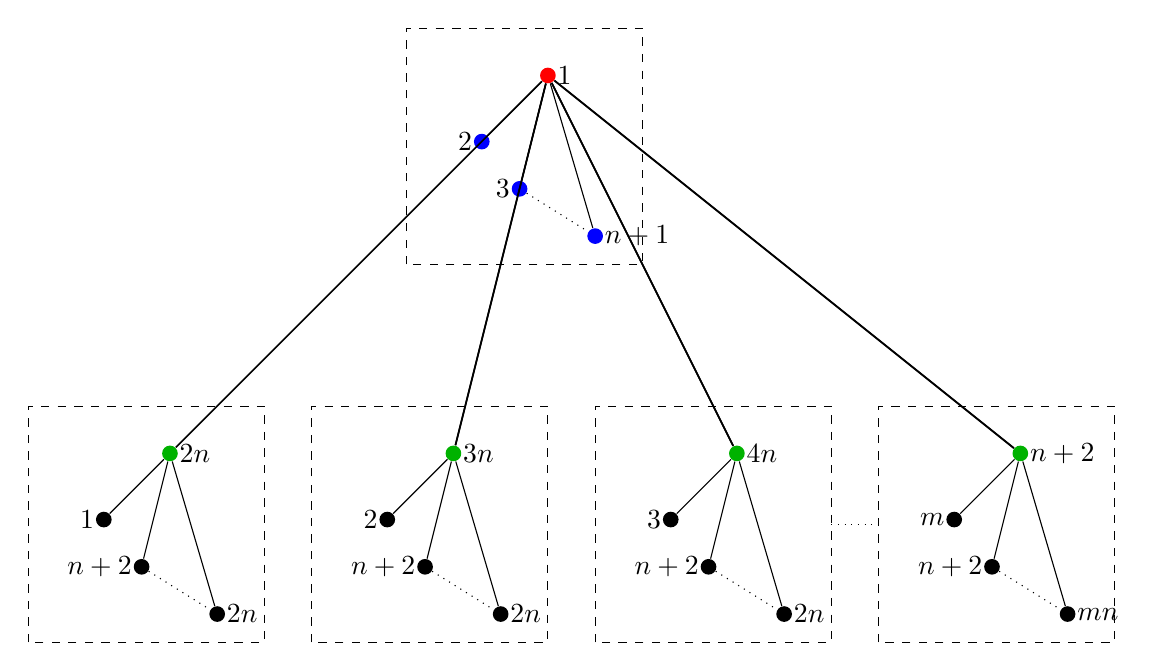
\begin{tikzpicture}[scale=1.2]
    % Define colors
    \colorlet{redcolor}{red}
    \colorlet{bluecolor}{blue}
    \colorlet{greencolor}{green!70!black}
    \colorlet{blackcolor}{black}
    
    % Top star graph (S_{1,n})
    \draw[dashed] (-1.5,4) rectangle (1,6.5);
    \node[circle, fill=redcolor, inner sep=2pt] (v0) at (0,6) {};
    \node[circle, fill=bluecolor, inner sep=2pt] (v1) at (-0.7,5.3) {};
    \node[circle, fill=bluecolor, inner sep=2pt] (v2) at (-0.3,4.8) {};
    \node[circle, fill=bluecolor, inner sep=2pt] (v3) at (0.5,4.3) {};
    
    % Edges in top star graph
    \draw (v0) -- (v1);
    \draw (v0) -- (v2);
    \draw (v0) -- (v3);
    
    % Dotted line indicating more vertices
    \draw[dotted] (v2) -- (v3);
    
    % Labels for top vertices
    \node[right] at (v0) {$1$};
    \node[left] at (v1) {$2$};
    \node[left] at (v2) {$3$};
    \node[right] at (v3) {$n+1$};
    
    % Bottom star graphs (copies of S_{1,n})
    % First copy
    \draw[dashed] (-5.5,0) rectangle (-3,2.5);
    \node[circle, fill=greencolor, inner sep=2pt] (w01) at (-4,2) {};
    \node[circle, fill=blackcolor, inner sep=2pt] (w11) at (-4.7,1.3) {};
    \node[circle, fill=blackcolor, inner sep=2pt] (w21) at (-4.3,0.8) {};
    \node[circle, fill=blackcolor, inner sep=2pt] (w31) at (-3.5,0.3) {};
    
    % Second copy
    \draw[dashed] (-2.5,0) rectangle (0,2.5);
    \node[circle, fill=greencolor, inner sep=2pt] (w02) at (-1,2) {};
    \node[circle, fill=blackcolor, inner sep=2pt] (w12) at (-1.7,1.3) {};
    \node[circle, fill=blackcolor, inner sep=2pt] (w22) at (-1.3,0.8) {};
    \node[circle, fill=blackcolor, inner sep=2pt] (w32) at (-0.5,0.3) {};
    
    % Third copy
    \draw[dashed] (0.5,0) rectangle (3,2.5);
    \node[circle, fill=greencolor, inner sep=2pt] (w03) at (2,2) {};
    \node[circle, fill=blackcolor, inner sep=2pt] (w13) at (1.3,1.3) {};
    \node[circle, fill=blackcolor, inner sep=2pt] (w23) at (1.7,0.8) {};
    \node[circle, fill=blackcolor, inner sep=2pt] (w33) at (2.5,0.3) {};
    
    % Fourth copy
    \draw[dashed] (3.5,0) rectangle (6,2.5);
    \node[circle, fill=greencolor, inner sep=2pt] (w04) at (5,2) {};
    \node[circle, fill=blackcolor, inner sep=2pt] (w14) at (4.3,1.3) {};
    \node[circle, fill=blackcolor, inner sep=2pt] (w24) at (4.7,0.8) {};
    \node[circle, fill=blackcolor, inner sep=2pt] (w34) at (5.5,0.3) {};
    
    % Edges in bottom star graphs
    % First copy
    \draw (w01) -- (w11);
    \draw (w01) -- (w21);
    \draw (w01) -- (w31);
    \draw[dotted] (w21) -- (w31);
    
    % Second copy
    \draw (w02) -- (w12);
    \draw (w02) -- (w22);
    \draw (w02) -- (w32);
    \draw[dotted] (w22) -- (w32);
    
    % Third copy
    \draw (w03) -- (w13);
    \draw (w03) -- (w23);
    \draw (w03) -- (w33);
    \draw[dotted] (w23) -- (w33);
    
    % Fourth copy
    \draw (w04) -- (w14);
    \draw (w04) -- (w24);
    \draw (w04) -- (w34);
    \draw[dotted] (w24) -- (w34);
    
    % Double lines connecting top and bottom star graphs
    \draw[line width=0.6pt] (v0) -- (w01);
    \draw[line width=0.6pt, yshift=1pt] (v0) -- (w02);
    \draw[line width=0.6pt, yshift=-1pt] (v0) -- (w02);
    \draw[line width=0.6pt, yshift=1pt] (v0) -- (w03);
    \draw[line width=0.6pt, yshift=-1pt] (v0) -- (w03);
    \draw[line width=0.6pt, yshift=1pt] (v0) -- (w04);
    \draw[line width=0.6pt, yshift=-1pt] (v0) -- (w04);
    
    % Labels for bottom vertices
    % First copy
    \node[right] at (w01) {$2n$};
    \node[left] at (w11) {$1$};
    \node[left] at (w21) {$n+2$};
    \node[right] at (w31) {$2n$};
    
    % Second copy
    \node[right] at (w02) {$3n$};
    \node[left] at (w12) {$2$};
    \node[left] at (w22) {$n+2$};
    \node[right] at (w32) {$2n$};
    
    % Third copy
    \node[right] at (w03) {$4n$};
    \node[left] at (w13) {$3$};
    \node[left] at (w23) {$n+2$};
    \node[right] at (w33) {$2n$};
    
    % Fourth copy
    \node[right] at (w04) {$n+2$};
    \node[left] at (w14) {$m$};
    \node[left] at (w24) {$n+2$};
    \node[right] at (w34) {$mn$};
    
    % Dots indicating more copies
    \draw[dotted] (3,1.25) -- (3.5,1.25);
\end{tikzpicture}

\end{document}